\section{Introduction}
As part of the investigations into VLS growth of CdTe nanowires, the control of the size and spatial distribution of metal seeds on oxides was investigated.
CdTe nanowire growth had been previously successful using Bi and BiTe seeds, however they are unstable, gold or another noble metal would expand the processing window both in terms of time and temperature.
As such, experiments into the control of gold on oxide substrates was undertaken.

While ultimately nanowire growth was suspended in favour of other investigations, the research into the interactions of gold overlayers on MgAl\(_2\)O\(_4\) (spinel) substrates yielded some surprising results.
The standard method of producing metal seed particles is thermal dewetting, relying upon the relative surface energies of metal versus substrate to cause the film to ball up.
The dewetting of gold on spinel substrates was found to result in epitaxial alignment and nanocrystal formation.
A full characterization into the formation process of the gold nanocrystals was undertaken and a phenomenological model of their formation was presented.
This work was published as ``Epitaxially driven formation of intricate supported gold nanostructures
on a lattice-matched oxide substrate'' in Nano Letters\cite{Devenyi2009}.
\section{Experimental}
The gold nanostructures were formed through the deposition of gold films on MgAl\textsubscript{2}O\textsubscript{4} substrates (MTI Corp.) followed by an annealing procedure which facilitated film dewetting and nanostructure formation.
The films were sputter-coated at room temperature to a thickness of 5--15~\AA{} with a GATAN PECS Model 682 ion beam coating/etching system.
The samples were then placed in a tube furnace with a 100~SCCM flow of argon, heated to 1100\celsius{} in 45~min, and then held at that temperature for 1~h.
Following this treatment, the sample was cooled to 1000\celsius{} in 30~min, held at that temperature for an additional hour, and then allowed to cool to room temperature over an interval of approximately 8~h.
Holding the temperature at both 1100 and 1000\celsius{} was crucial to the formation of the nanostructures described here.
Removal of either step results in the formation of faceted gold spheres sitting directly on the substrate.

Scanning electron microscopy (SEM) images of the gold nanostructures formed on the (100), (111), and (110) MgAl\textsubscript{2}O\textsubscript{4} substrates, obtained using a JEOL-7000F SEM in secondary electron mode, are shown in \cref{fig:nanogold_sem}.
For each substrate orientation, one observes two types of features, (i) spheres supported by a necking region attached to a geometrically shaped base (\cref{fig:nanogold_sem}a-c) and (ii) standalone base structures (\cref{fig:nanogold_sem}d-f).
Convergent beam electron diffraction (CBED) performed using a Phillips CM12 confirmed that the supported spheres are crystalline.
For each case, the shape of the base structure reflects the underlying symmetry of the substrate which is four-fold, three-fold, and two-fold symmetric for the (100), (111), and (110) surfaces.
X-ray diffraction measurements, using a Bruker 6000 CCD detector on a Bruker three circle D8 goniometer with a Rigaku RU-200 rotating anode Cu KR X-ray generator and parallel-focusing mirror optics, were used to determine the substrate orientation relative to the edges of the base structures and are denoted on the three top-down SEM images (\cref{fig:nanogold_sem}d-f).
\section{Results and Discussion}
The crystallographic alignment of the nanostructures is a clear indication of epitaxy and is strongly suggestive of {111} gold faceting of the base structures associated with the [100]- and [111]-oriented substrates.
For the (110) surface, the standalone base structures are ill-defined and show no obvious faceting, while those formed in combination with a sphere show shapes consistent with mixed faceting, possibly having \{111\} and \{100\} facets for the short and long dimension.
The standalone base dimensions are uniform with side lengths of 40, 65, and 65~nm \(\times\) 110~nm for the (100), (111), and (110) substrates.
\begin{figure}
 \centering 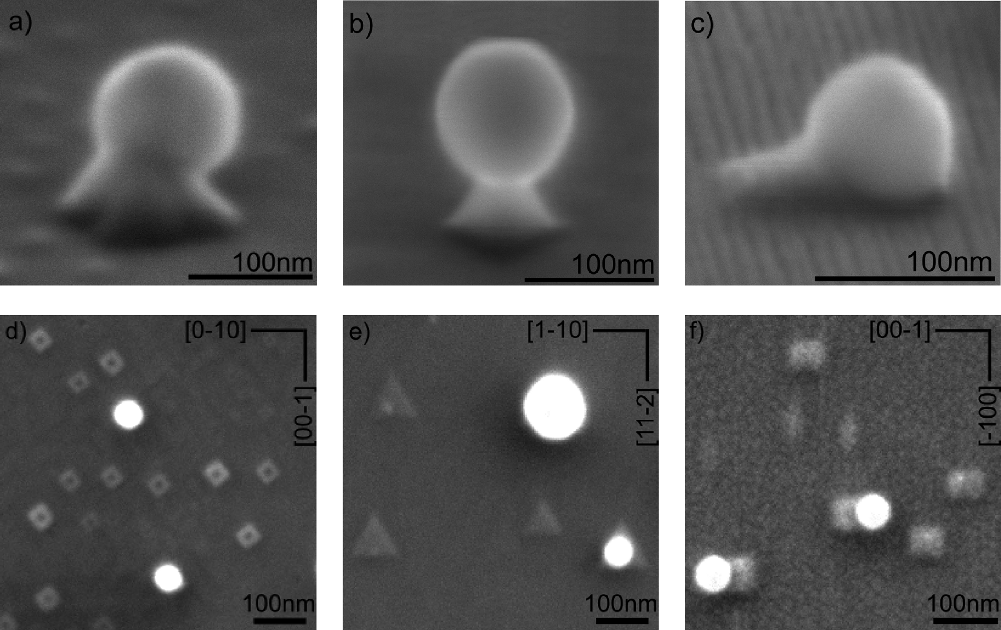
\includegraphics[width=0.8\textwidth]{nanogold_sem}
 \caption[SEM images of gold nanostructures]{\label{fig:nanogold_sem}SEM images showing the gold nanostructures formed on MgAl\textsubscript{2}O\textsubscript{4} substrates.
  The three upper images show spheres supported by a necking region attached to a geometrically shaped base for the (a) [100]-, (b) [111]-, and (c) [110]-oriented substrates.
  Each of these images was taken at a 70\degree tilt.
  The aura seen around nanostructures is an artifact of imaging.
  The three lower images show the top-down view of both standalone base structures and supported spheres for the (d) [100]-, (e) [111]-, and (f) [110]- oriented substrates.
  The in-plane Miller indices of the substrate are denoted on each of these images.
  For all cases, the samples were coated with a thin layer of platinum to improve imaging.
  Imaging without platinum shows the same structures but is of poor quality due to substrate charging effects.}
\end{figure}

While there are two basic types of nanostructures formed on each substrate orientation, these structures are found in various stages of development.
For the most part, the bases are well-developed and show little size variation.
The spherical structures, however, vary dramatically both in their size and position relative to the base structures.
\cref{fig:nanogold_progression} shows a series of top-down SEM images for the case of the (111) MgAl\textsubscript{2}O\textsubscript{4} substrate showing an evolution of the nanostructures from a standalone triangular base to bases supporting spheres of increasing size.
Notable is the fact that the nanostructure, shown in \cref{fig:nanogold_progression}b, manifests itself as a small sphere which is offset from the centre of the base while for the larger spheres, this asymmetry disappears.
Such asymmetries are observed for all three substrate orientations, but only those nanostructures formed on the (111) substrate consistently show a centrally placed sphere for the large sphere sizes.
There is also a systematic effect whereby the size of the triangular base structure increases for sphere diameters greater than 80~nm (see \cref{fig:nanogold_progression}e and f).
\begin{figure}
 \centering 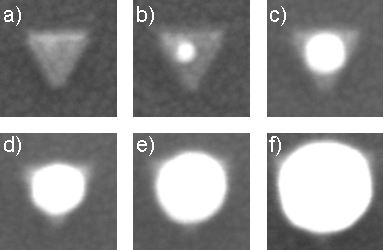
\includegraphics[width=0.9\textwidth]{nanogold_progression}
 \caption[SEM of gold nanostructure growth progression]{\label{fig:nanogold_progression}SEM images showing the top-down view of gold nanostructures formed on the (111) surface of MgAl\textsubscript{2}O\textsubscript{4} substrates.
  The sequence of images is chosen to show progressively larger spheres atop the base structures.
  Only the smallest sphere, shown in b), is offset from the centre of the triangular base and that the base size is slightly larger when supporting larger spheres, as happens for e) and f).
  The size of each image is 130\(\times\)30~nm\textsuperscript{2}.}
\end{figure}

The base structures formed on each substrate orientation are a clear consequence of the epitaxial relationship formed between gold and the latticed-matched MgAl\textsubscript{2}O\textsubscript{4} substrate.
This is apparent from the fact that the geometries of the base structures mimic the underlying symmetry of the substrates.
It is also likely that the base sizes are a consequence of the substrate-imposed strains.
Arguments based on epitaxy, however, cannot explain the self-assembly of the gold spheres atop the base structures and the associated necking behaviour which facilitates their connection to the base.
It is our hypothesis that the necking behaviour results from an attempt to minimize the surface energy of the structure.
Thus, the overall shape of these nanostructures is governed by an interplay between the constraints imposed by epitaxy and a requirement that the surface free energy be minimized.
This situation has much in common with formation of soap bubbles affixed to a wire frame\cite{RefWorks:95}.
This statement is based on the facts that the frame imposes a constraint analogous to that imposed by lattice mismatch and that the shape of the soap bubble is, to a large degree, determined by the surface free energy.
This analogy provided the impetus for applying the well-developed models associated with soap bubble formation to the nanostructures described here.
Such modelling has also been successfully used to predict the equilibrium shape of biological lipid bilayers (blood cells) when exposed to abnormal pressure, temperature, magnetic, and chemical environments\cite{RefWorks:99,RefWorks:102,RefWorks:47,RefWorks:100,RefWorks:101,RefWorks:103}.

The gold nanostructures were modelled as a continuum elastic surface constrained by a footprint.
Three different footprint geometries (square, equilateral triangle, and rectangle) were used in order to mimic the four-fold, three-fold, and two-fold symmetries associated with the (100), (111), and (110) surfaces of MgAl\textsubscript{2}O\textsubscript{4}.
The size and shape of the footprint were kept constant during the simulated growths in order to match the experimental observation indicating a high degree of base uniformity.
For each orientation, the contact angle (i.e., the angle between the footprint plane and the tangent plane of any surface connected to the footprint's edge) was set to a constant where the value was chosen to be consistent with the observed faceting, as is schematically shown in \cref{fig:nanogold_facets}.

With these constraints, the shape of an open elastic surface can be fully described by the mean curvature, H, and the Gaussian curvature, \textbf{K}, while its corresponding elastic properties can be characterized by a bending modulus \textkappa and a Gaussian modulus \textkappa\textsubscript{G}.
The surface energy (\(F\)) can then be formulated as
\begin{equation}
 F = \int \frac{\kappa}{2}H^2 dA + \int \kappa_G K dA + \lambda S + PV \label{nanogold:eqn1}
\end{equation}
where \textlambda, \textbf{V}, \textbf{S}, and \textbf{dA} are the particle's surface tension, volume, total surface area, and surface area element\cite{RefWorks:49,RefWorks:97}.
The pressure, \textbf{P}, serves as a Lagrange multiplier which ensures that a constant volume is enclosed between the structure and the footprint plane.
The second term gives the integrated Gaussian curvature, which is constant according to the Gauss-Bonnet theorem\cite{RefWorks:98}.
For a given surface tension and volume, the equilibrium shape will correspond to an energy minimum determined by the shape equation \textdelta{} \textbf{F} \(=\) 0.
The structures are more readily solved by first rescaling the free energy of the model to become dimensionless, such that
\begin{equation}
 \tilde{F} = \int \left (\frac{\tilde{\kappa} \tilde{H}^2}{2} + 1 \right)d \tilde{A} + \tilde{P} \tilde{V} \label{nanogold:eqn2}
\end{equation}
where
\begin{align*}
 \tilde{A} &%
 = A/S_0 & \tilde{V} &%
 = V/S^{3/2}_0 &
 \tilde{H} &%
 = H S^{1/2}_0 \\
 \tilde{\kappa} &%
 = \kappa / \lambda S_0 &
 \tilde{P} &%
 = P S^{1/2}_0 / \lambda &
 \tilde{F} &%
 = F / (\lambda S_0)
\end{align*}
and \textbf{S\textsubscript{0}} is the area of the base.
Thus, according to this dimensionless free-energy expression, there are two independent controlling parameters, \(\tilde{\kappa}\) and \textbf{P}.

Helfrich and Ou-Yang\cite{RefWorks:49} have analytically solved the shape equation for some symmetrical geometries.
For the work presented here, the surface is sectioned into discrete elements using a triangulation mesh, and a simple dissipative model is used to minimize the energy, as in \cref{nanogold:eqn2}\cite{RefWorks:76}
\begin{equation}
 \frac{\delta \mathbf{r}}{\delta t} = - M \frac{\delta \tilde{F}}{\delta \mathbf{r}} \label{nanogold:eqn3}
\end{equation}
where \textbf{r(t)} is the position vector of a point on the particle surface at time \textbf{t} and \textbf{M} is a kinetic coefficient.
These methods, developed by Taniguchi et al.\cite{RefWorks:76}, are, however, unable to simulate large deformations.
To circumvent this limitation, we employed two techniques, equiangulation and vertex averaging, available through the Surface Evolver software developed by Brakke et al.\cite{RefWorks:62}. Following the procedure of Lim et al.,\cite{RefWorks:99,RefWorks:100,RefWorks:101} the curvature was discretized based on the methods of Julicher\cite{RefWorks:52}, which exactly describe the curvature in the continuum limit.

The variational derivative used in the triangulation scheme was evaluated analytically.
For the Surface Evolver technique, variables were solved numerically when analytical variations for discrete curvatures proved difficult.
\begin{figure}
 \centering 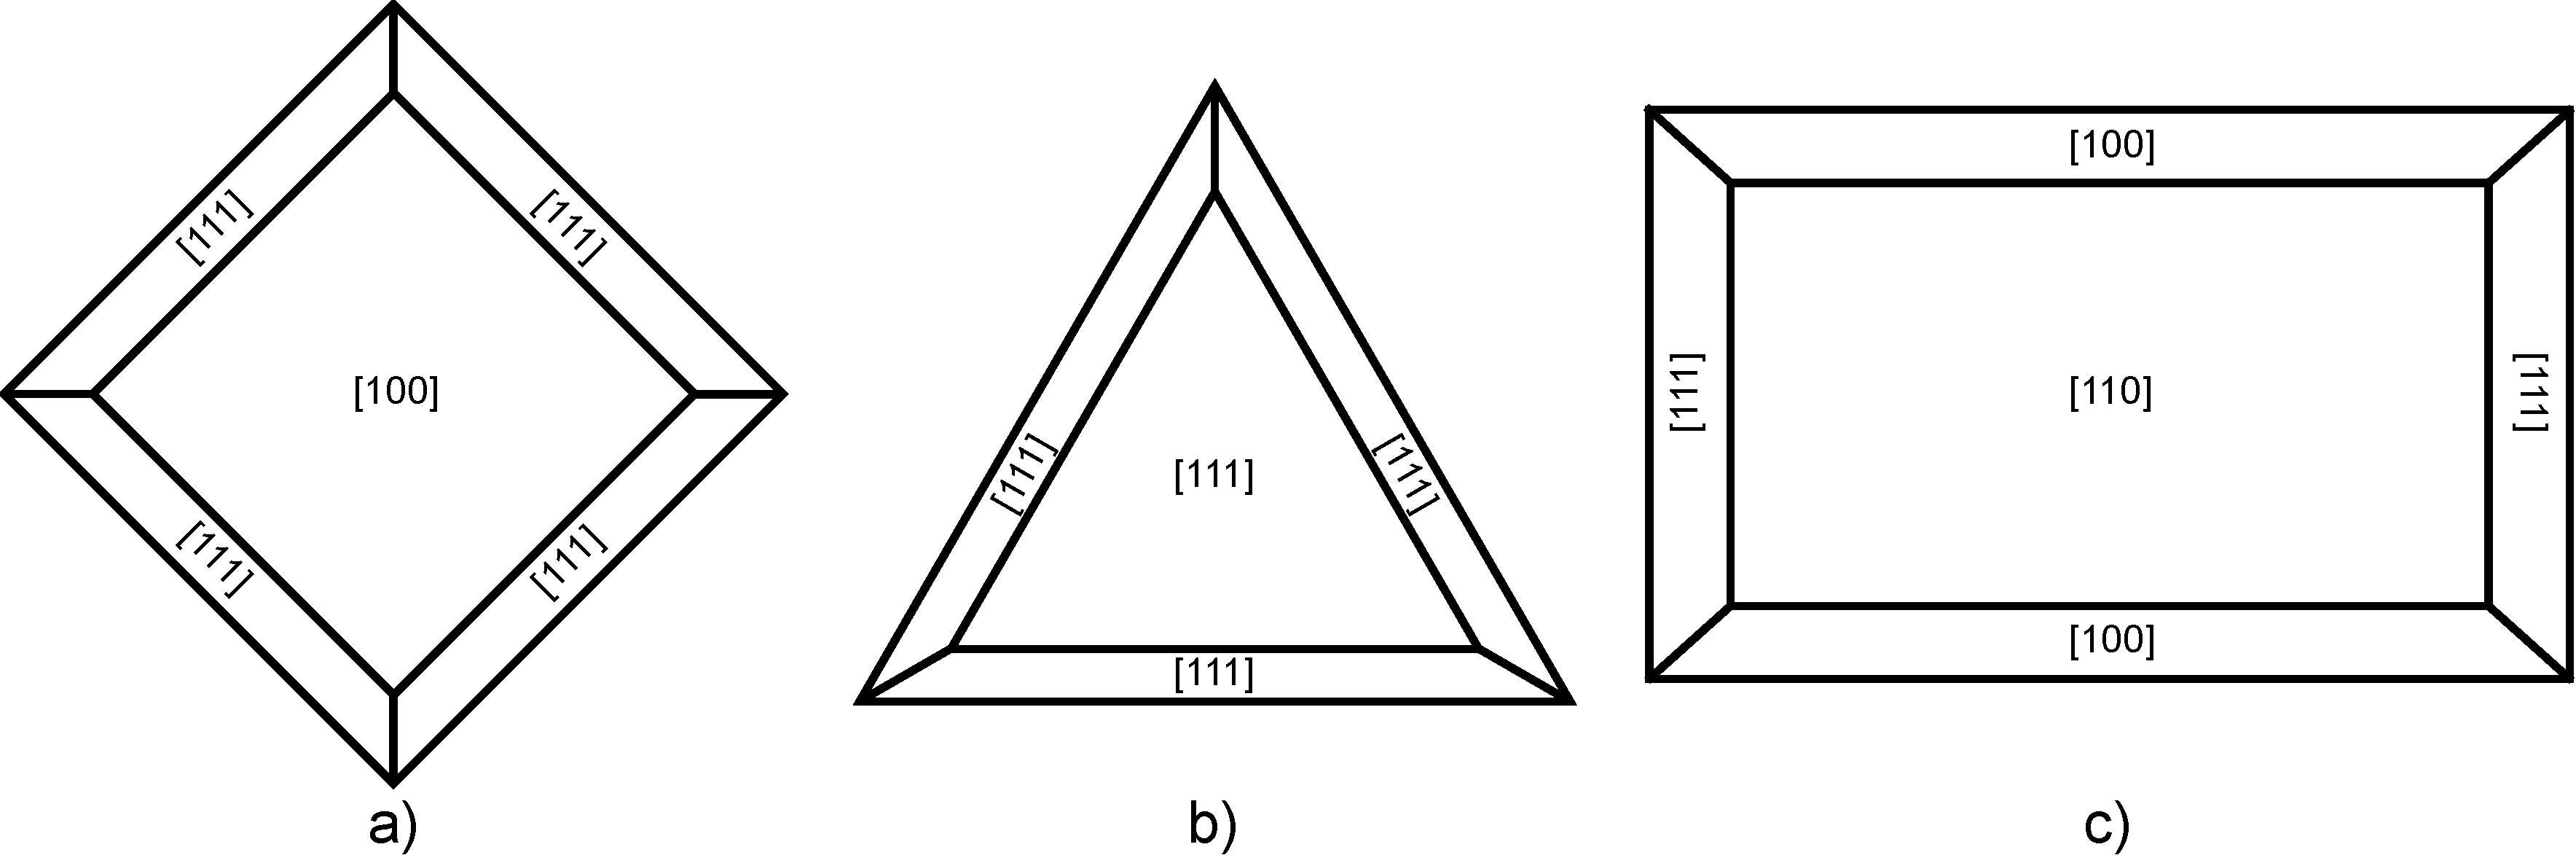
\includegraphics[width=\textwidth]{nanogold_facets}
 \caption[Model of gold nanostructure faceting]{\label{fig:nanogold_facets}Proposed faceting of the base structures grown on (a) [100]-, (b) [111]-, and (c) [110]-oriented substrates.}
\end{figure}
\begin{figure}
 \centering 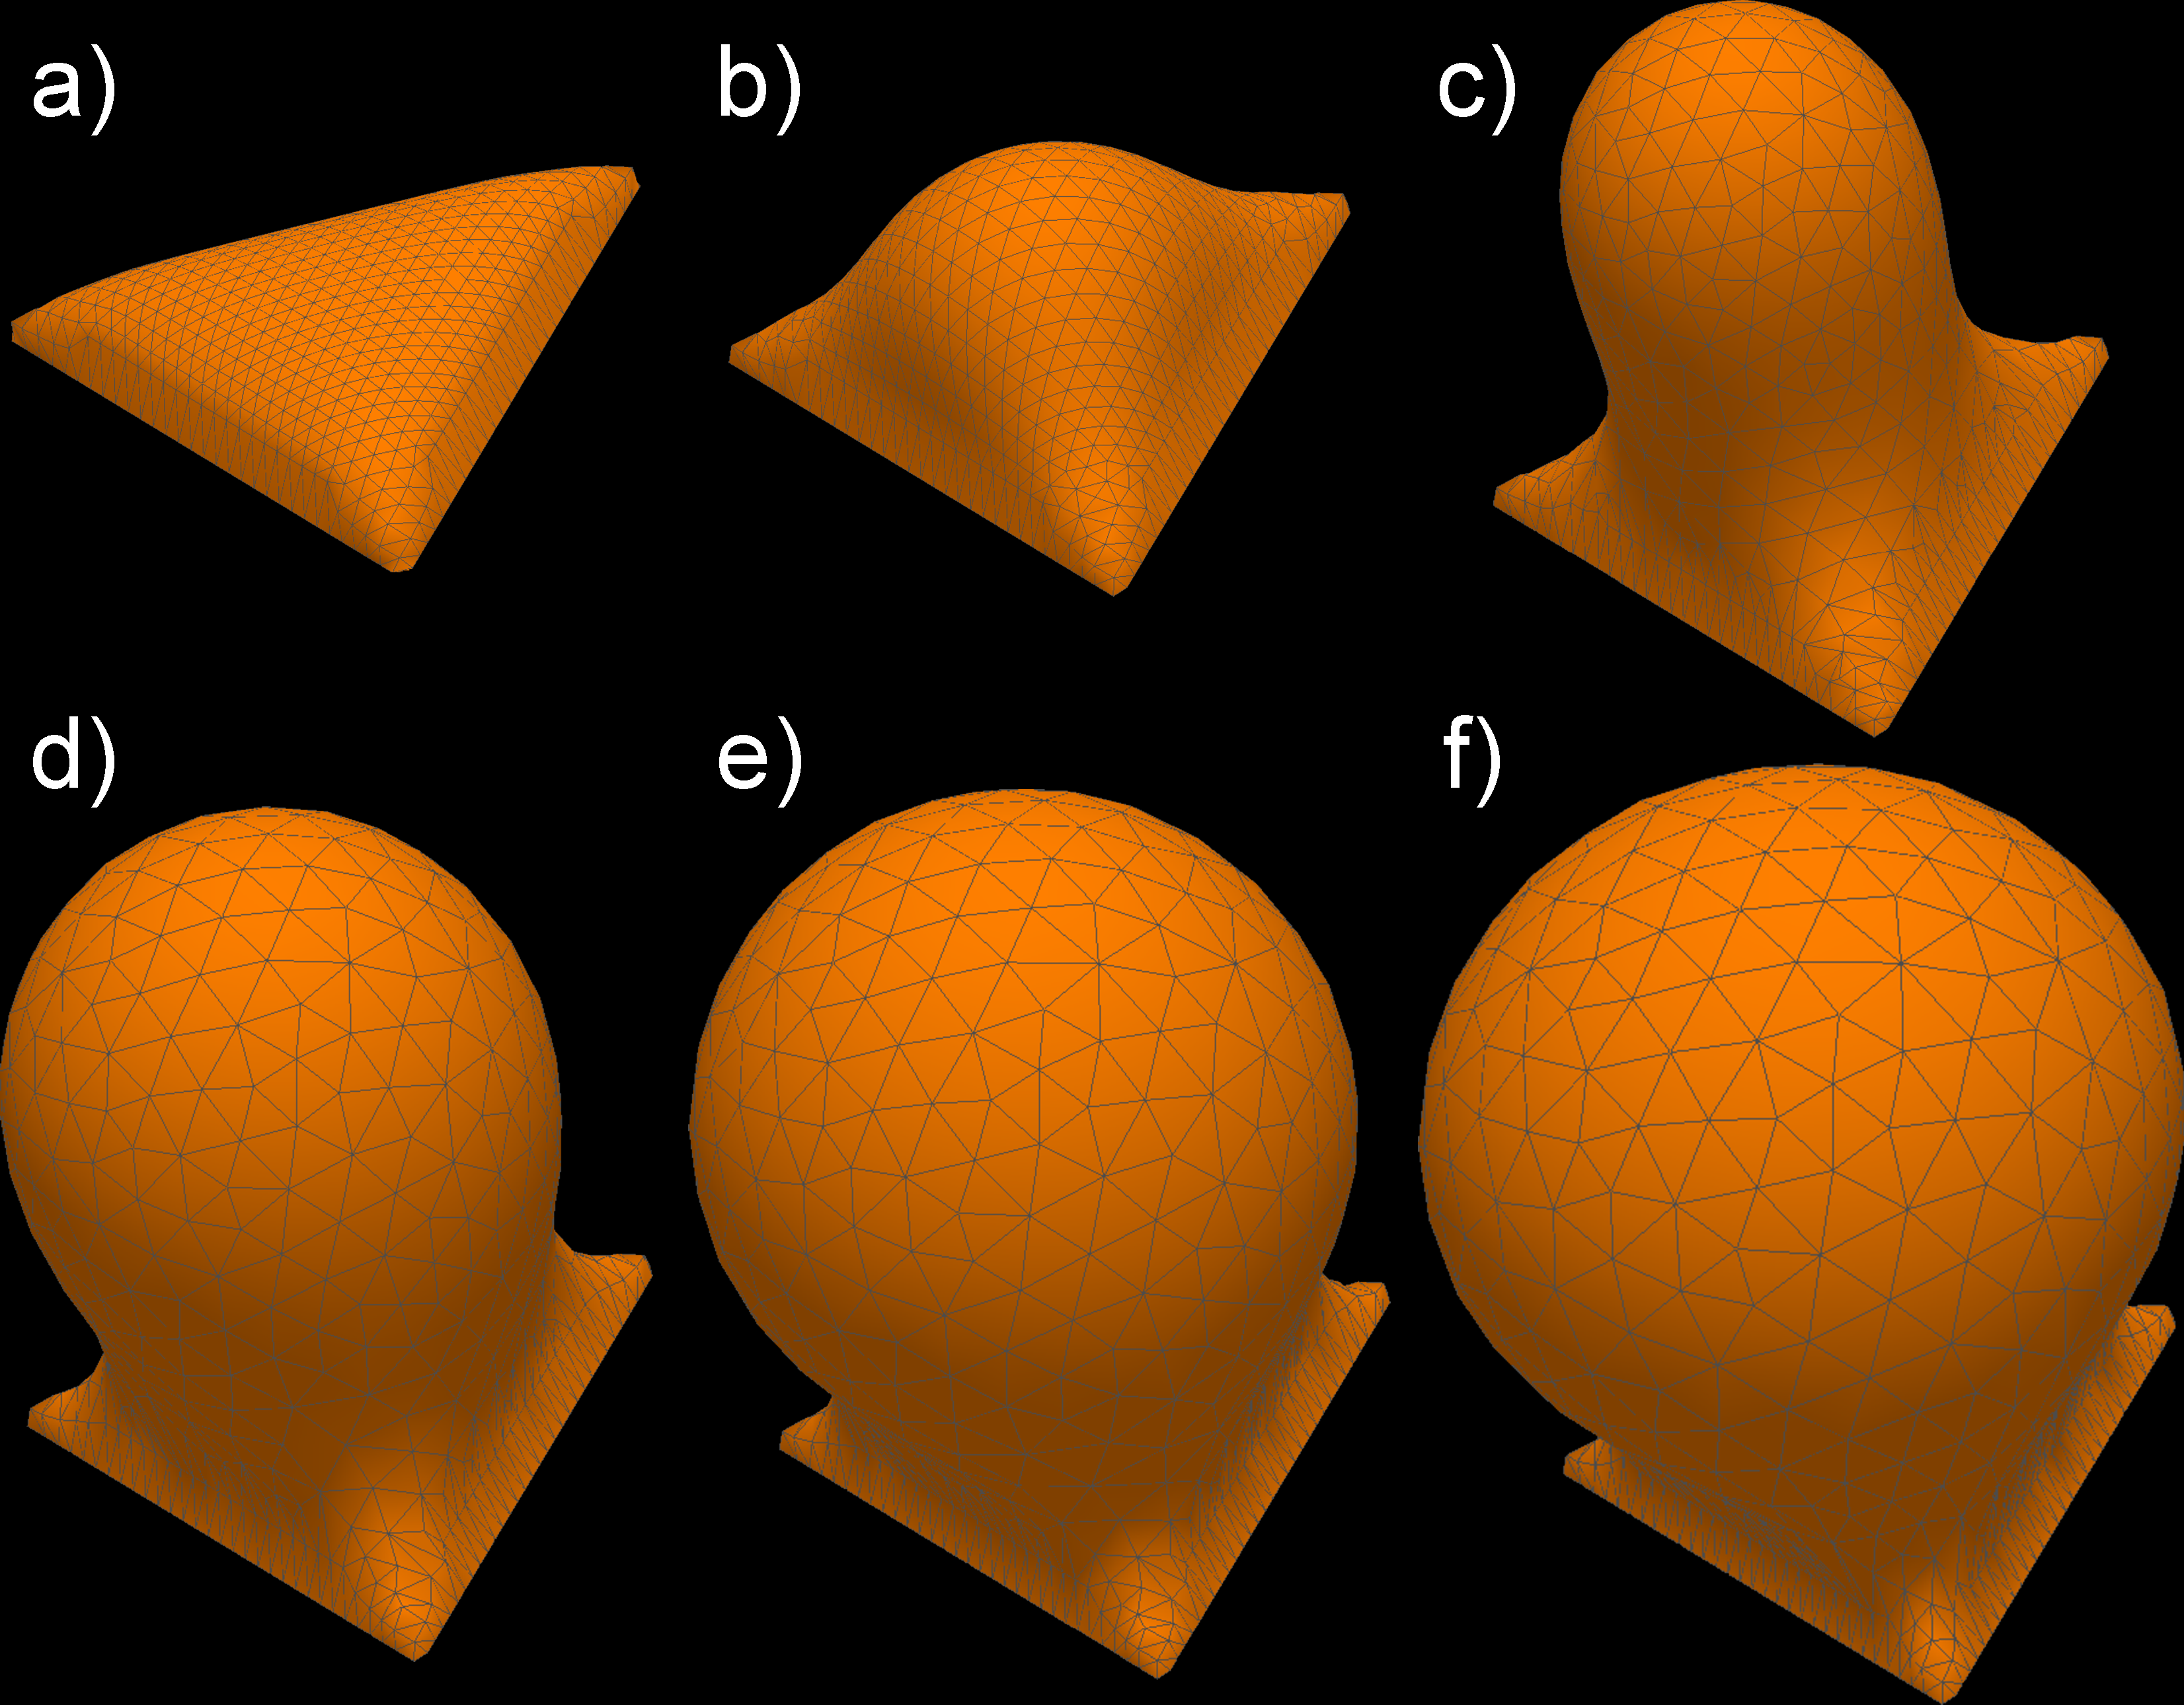
\includegraphics[width=\textwidth]{nanogold_simgrowth}
 \caption[Simulated gold nanostructure growth]{\label{fig:nanogold_simgrowth}Simulations based on the continuum elastic model showing the shape evolution of structures with a triangular footprint as the total volume is progressively increased.
  The shape of these modelled structures resembles that of the self-assembled gold nanostructures formed on (111) MgAl\textsubscript{2}O\textsubscript{4} substrates (\protect{\cref{fig:nanogold_sem}}b and e and \protect{\cref{fig:nanogold_progression}}).
  The scale is in arbitrary units.}
\end{figure}

Using the numerical methodology, a progression of structures with increasing volume were calculated using square, triangular, and rectangular footprints having contact angles of 54.7\degree, 70.5\degree, and 35\degree{} (long-axis) by 45\degree{} (short-axis).
The chosen contact angles are consistent with the inferred faceting, as shown in \cref{fig:nanogold_facets}.
For each case, the footprint area and surface tension are set to unity, while the bending modulus is allowed to vary.
\cref{fig:nanogold_simgrowth} shows the calculated progression for the triangular footprint.
As the volume is increased, there is an evolution from a nearly flat base, to a base with a bulge, and then finally to a spherical structure supported by a necked region to a triangular base.
These simulated structures are similar to the gold nanostructures formed on the (111) MgAl\textsubscript{2}O\textsubscript{4} substrate (see \cref{fig:nanogold_sem}b and c and \cref{fig:nanogold_progression}).
Similar trends are observed for the square and rectangular footprints.
\Cref{fig:nanogold_square_rect} shows the simulated high volume structures for the square and rectangular footprints, which, once again, are consistent with experimental observations.
The simulations do not, however, account for any of the observed asymmetries.
\begin{figure}
 \centering 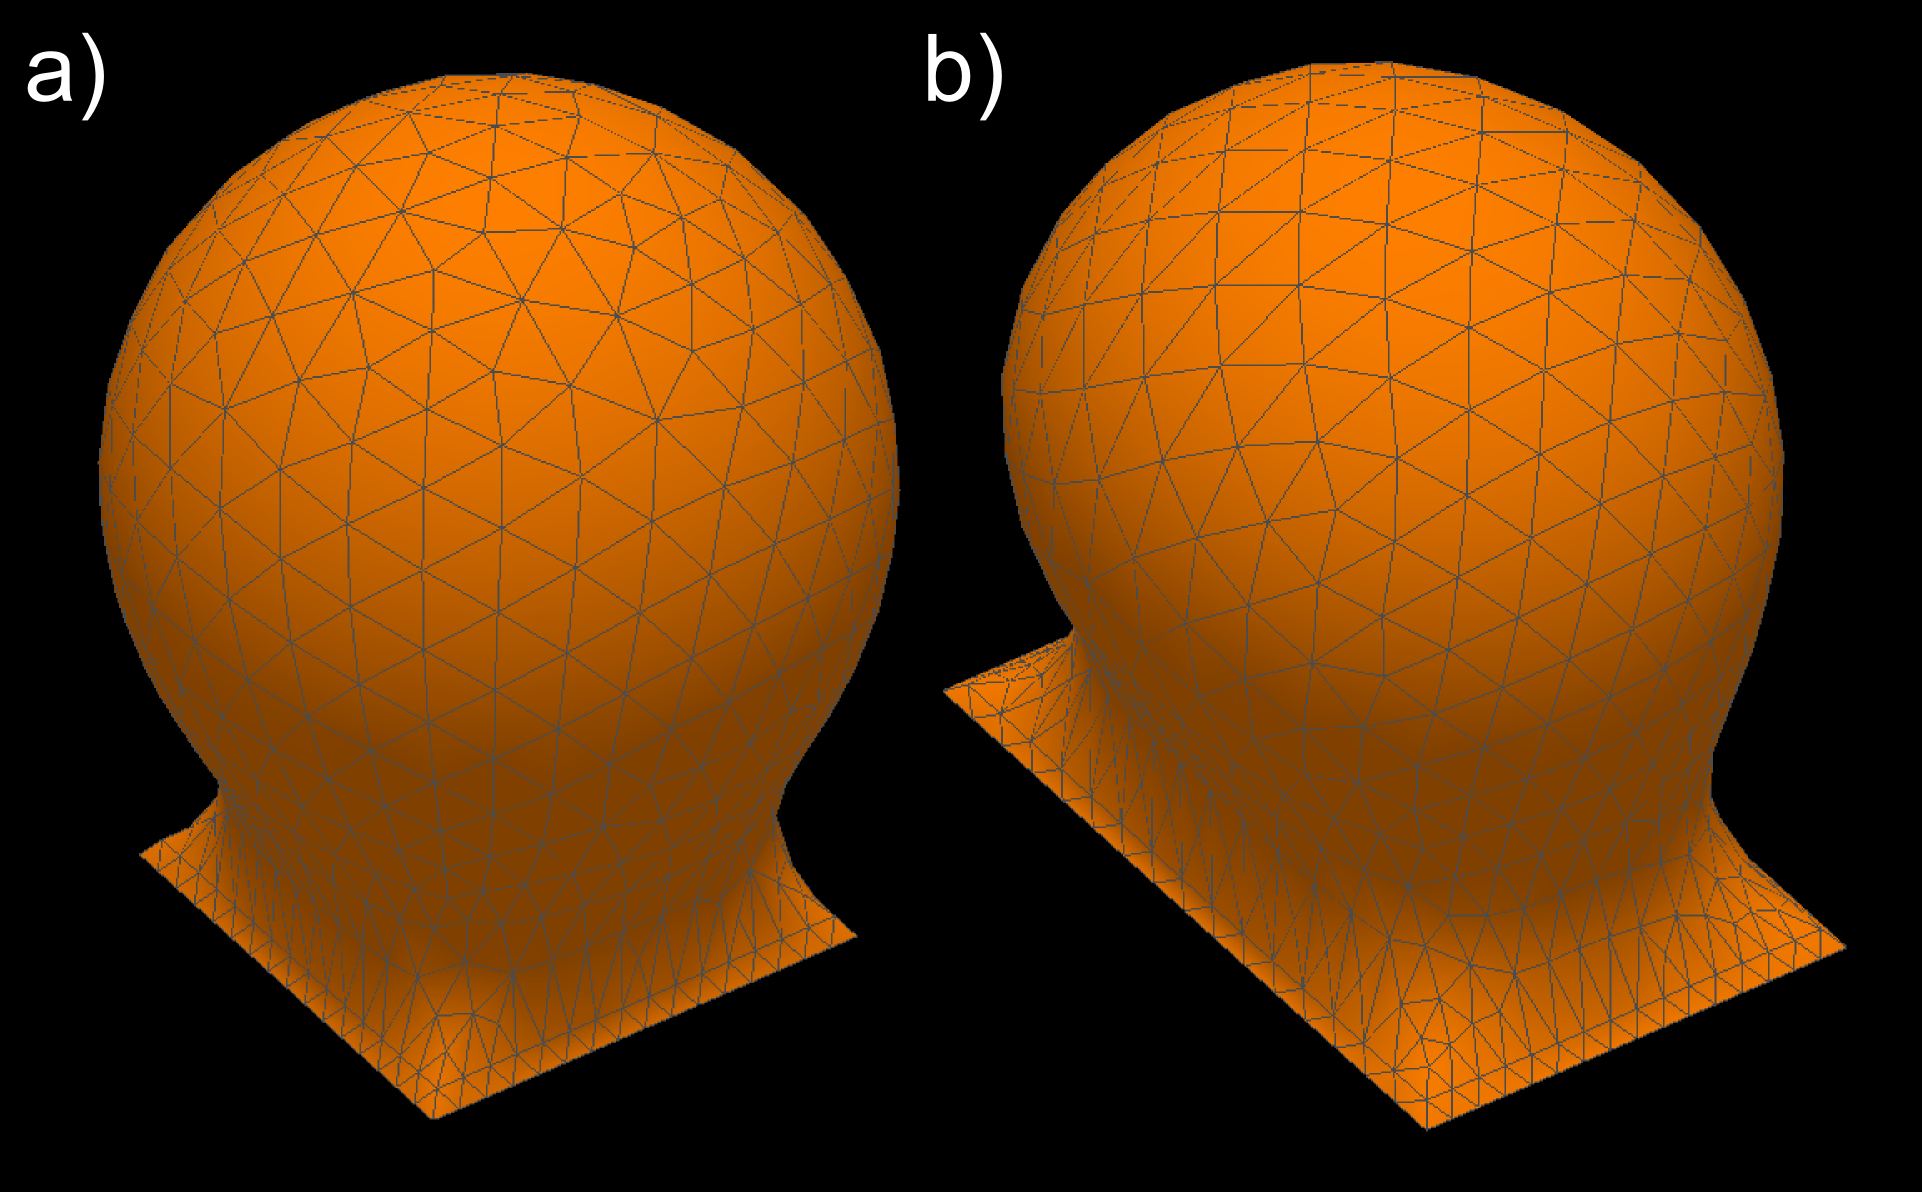
\includegraphics[width=\textwidth]{nanogold_square_rect}
 \caption[Simulations of square and rectangular base gold nanostructures]{\label{fig:nanogold_square_rect}Simulations based on the continuum elastic model showing the expected high volume shape for the (a) square and (b) rectangular (length:width) 1.42:1 footprints.
  These structures show a resemblance to the self-assembled gold nanostructures formed on the (100) and (110) MgAl\textsubscript{2}O\textsubscript{4} substrates (\protect{\cref{fig:nanogold_sem}}) but show none of the observed asymmetries.
  The scale is in arbitrary units.}
\end{figure}

The shape of the base structures of the self-assembled gold nanostructures is strongly influenced by epitaxy and the underlying symmetry of the substrate surface.
That being said, it is difficult to account for the hollowed-out center observed for the base structure formed on the (100) MgAl\textsubscript{2}O\textsubscript{4} using epitaxy-based arguments.
This feature is, however, predicted by the continuum elastic model.
\Cref{fig:nanogold_afm}a shows the topographical color map obtained from the modelling for the low-volume structure.
It shows a circular depression in the middle of the structure as well as a lobe near each corner.
Motivated by the simulation results, we examined the topography of the self-assembled gold nanostructure using atomic force microscopy (AFM).
\Cref{fig:nanogold_afm}b shows a tapping mode AFM image of the base structure obtained using a Digital Instruments scanning probe microscope (SPM) and a NanoScope IIIa controller.
Even though the features of the nanostructure are somewhat washed out since the resulting image is a convolution of the nanostructure and the AFM tip geometry, the nanostructure's four lobes and central depression are visible.
\begin{figure}
 \centering 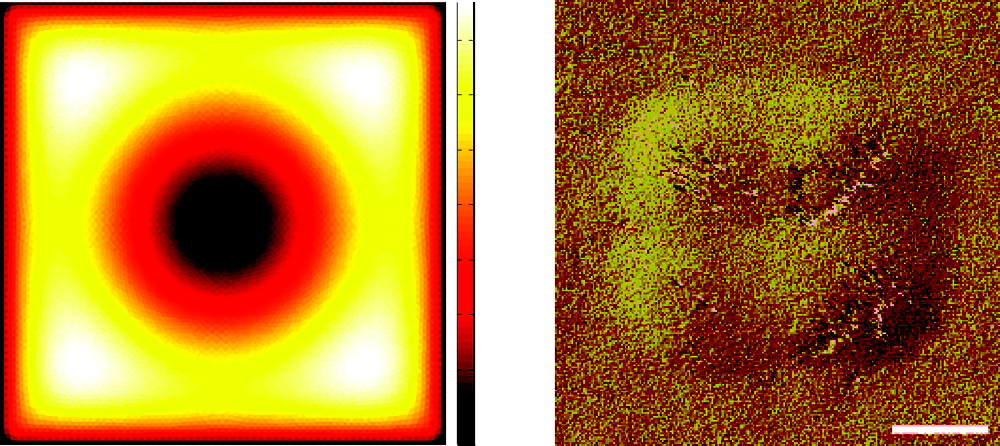
\includegraphics[width=0.8\textwidth]{nanogold_afm}
 \caption[Comparison of AFM and simulated gold nanostructure topography]{\label{fig:nanogold_afm}A comparison of the (a) topographical colour map derived from the continuum elastic model and (b) the AFM image of a self-assembled gold nanostructure deposited on the (100) MgAl\textsubscript{2}O\textsubscript{4} substrate.
  The simulation predicts both the presence of four lobes at the corners and a central depression.
  The scale of the topographic image is arbitrary, and the scale of the AFM image is 10~nm.}
\end{figure}

Taken together, the experimental observations and the continuum elastic modelling results strongly suggest that epitaxy and a minimization of the surface free energy are the two primary drivers in determining the shape and size of the self-assembled gold nanostructures.
The fact that similar structures have not been previously observed is likely a consequence of the synthesis route used.
The route employed here not only involves temperatures well in excess of those typically used when forming substrate-supported nanostructures but also requires an annealing profile which accesses two temperatures.
It is possible that the initial 1100\celsius{} anneal is needed to induce surface reconstructions in the MgAl\textsubscript{2}O\textsubscript{4} substrates which are essential to the growth of these nanostructures.
Surface reconstructions have been shown to strongly influence the growth of both nanostructures\cite{RefWorks:24,RefWorks:16,RefWorks:104} and thin films\cite{Neretina2009a} when using (100) SrTiO3 substrates.
We, however, consider it more likely that the formation of these nanostructures requires temperatures in excess of the melting point of bulk gold (1064\celsius{}).
Significant deviations from the bulk value, due to finite size effects, are considered unlikely since such effects appear to occur only in nanostructures smaller than 5~nm\cite{RefWorks:43}.
Once molten, the nanostructures are cooled to 1000\celsius{} and held at this temperature, which is just below the melting point.
Such a temperature allows for solidification while maintaining high adatom mobility.
The fact that this fabrication step is crucial to the formation of the observed intricate nanostructures provides compelling evidence that substantial adatom motion is essential.
In this scenario, it is likely that an Ostwald-like ripening process will play a role where larger nanostructures grow at the expense of smaller ones.
Substrate surface steps, due to the inherent miscut of the substrate\cite{RefWorks:69}, could also influence the process by providing energetically favourable nucleation sites.
Nanostructure formation is also heavily reliant on the epitaxial relationship between the nanostructure base and the underlying substrate.
This relationship determines the crystallographic alignment of the base structures, while the consistency in size is likely a consequence of the strain imposed by lattice mismatch.
Once the 1000\celsius{} anneal ends, the adatom motion will be quickly quenched by the lower temperatures, allowing no further alterations to the shape or size of the nanostructures.
The result is intricately shaped nanostructures whose size and shape are determined by a minimization of the surface free energy while simultaneously being subject to the constraints imposed by epitaxy.
\section{Implications for Symmetry and Energy at Epitaxial Surfaces}
Despite the materials of interest in this investigation consisting of a noble metal and a complex oxide, materials which one would not expect any kind of interaction, result in epitaxial alignment.
This epitaxial alignment is simple in the sense that the nanocrystal orientations follow directly from the underlying substrate.
The epitaxial alignment is complicated by the fact that gold fits onto sublattice of half of a MgAl\textsubscript{2}O\textsubscript{4} lattice.
Such epitaxy relies on the symmetry of the surface atoms forming a lattice with a smaller lattice constant than the bulk crystal.
This epitaxy can thus be thought of as nanocrystal forming on a reconstructed surface, since the surface atoms present a surface net with a different lattice parameter than the bulk.

The more surprising result from this work is the epitaxial alignment possible between nonreactive materials.
Noble metals are not known to readily react with other elements or compounds other than to form simple metallic bonds.
Similarly, metals overall are not known to strongly wet oxide surfaces, preferring to bond to themselves instead.
Complex oxides are also known to be stable to high temperatures, and stable when exposed to reactive compounds.
To mix such two compounds and observe something other than segregation and no interaction is surprising.
These experiments have shown that, despite there being a weak interaction between the two materials, due to low reactivity, epitaxial alignment is achieved through a careful thermal treatment.
The subtle influence of the substrate's lattice can impart alignment of the gold, overriding the tendency to form an equilibrium crystal shape.
